\documentclass{standalone}
\usepackage{tikz}
\usetikzlibrary{patterns, positioning}

\begin{document}
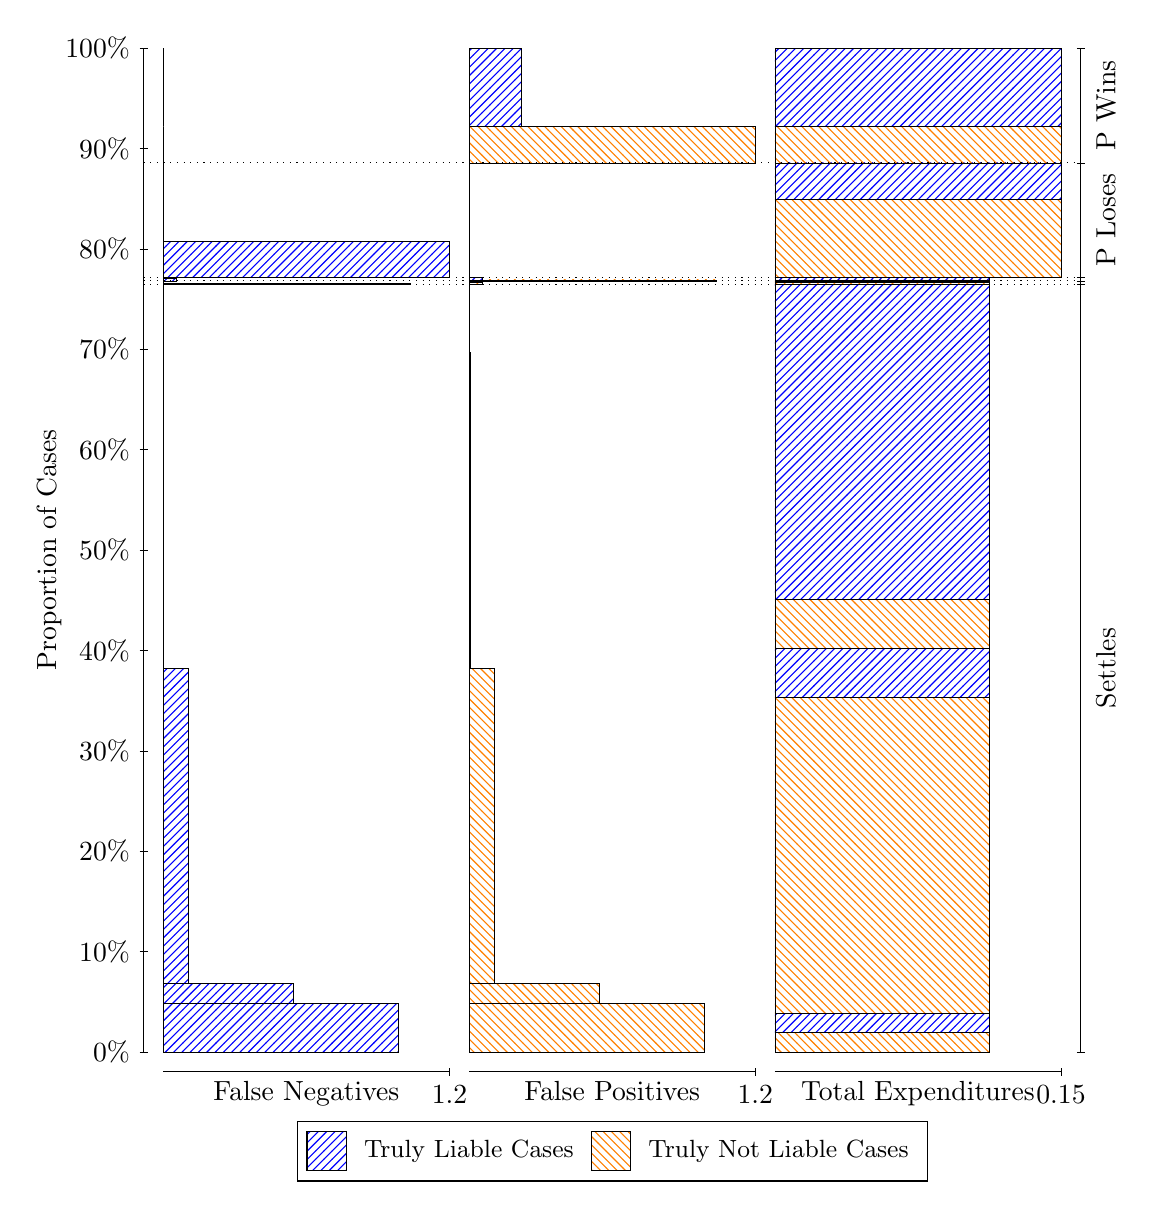
\begin{tikzpicture}
\draw[black, very thin] (1.5,1.75) -- (1.5,14.5);
\node[rotate=90, anchor=center] at (0.3, 8.125) {Proportion of Cases};
\draw[black, very thin] (1.45,1.75) -- (1.55,1.75);
\node[anchor=east] at (1.45, 1.75) {0\%};
\draw[black, very thin] (1.45,3.025) -- (1.55,3.025);
\node[anchor=east] at (1.45, 3.025) {10\%};
\draw[black, very thin] (1.45,4.3) -- (1.55,4.3);
\node[anchor=east] at (1.45, 4.3) {20\%};
\draw[black, very thin] (1.45,5.575) -- (1.55,5.575);
\node[anchor=east] at (1.45, 5.575) {30\%};
\draw[black, very thin] (1.45,6.85) -- (1.55,6.85);
\node[anchor=east] at (1.45, 6.85) {40\%};
\draw[black, very thin] (1.45,8.125) -- (1.55,8.125);
\node[anchor=east] at (1.45, 8.125) {50\%};
\draw[black, very thin] (1.45,9.4) -- (1.55,9.4);
\node[anchor=east] at (1.45, 9.4) {60\%};
\draw[black, very thin] (1.45,10.675) -- (1.55,10.675);
\node[anchor=east] at (1.45, 10.675) {70\%};
\draw[black, very thin] (1.45,11.95) -- (1.55,11.95);
\node[anchor=east] at (1.45, 11.95) {80\%};
\draw[black, very thin] (1.45,13.225) -- (1.55,13.225);
\node[anchor=east] at (1.45, 13.225) {90\%};
\draw[black, very thin] (1.45,14.5) -- (1.55,14.5);
\node[anchor=east] at (1.45, 14.5) {100\%};

\draw[black, very thin] (13.4,1.75) -- (13.4,14.5);
\draw[black, very thin] (13.35,1.75) -- (13.45,1.75);
\node[anchor=west] at (13.35, 1.75) {};
\draw[black, very thin] (13.35,11.5) -- (13.45,11.5);
\node[anchor=west] at (13.35, 11.5) {};
\draw[black, very thin] (13.35,11.542) -- (13.45,11.542);
\node[anchor=west] at (13.35, 11.542) {};
\draw[black, very thin] (13.35,11.584) -- (13.45,11.584);
\node[anchor=west] at (13.35, 11.584) {};
\draw[black, very thin] (13.35,13.042) -- (13.45,13.042);
\node[anchor=west] at (13.35, 13.042) {};
\draw[black, very thin] (13.35,14.5) -- (13.45,14.5);
\node[anchor=west] at (13.35, 14.5) {};

\draw[black, very thin, pattern color=blue, pattern=north east lines] (1.75,1.75) rectangle (4.7345,2.3718);
\draw[black, very thin, pattern color=blue, pattern=north east lines] (1.75,2.3718) rectangle (3.3998,2.6185);
\draw[black, very thin, pattern color=blue, pattern=north east lines] (1.75,2.6185) rectangle (2.0651,6.6249);
\draw[black, very thin, pattern color=orange, pattern=north west lines] (1.75,6.6249) rectangle (1.75,11.5);
\draw[black, very thin, pattern color=blue, pattern=north east lines] (1.75,11.5) rectangle (4.8828,11.513);
\draw[black, very thin, pattern color=orange, pattern=north west lines] (1.75,11.513) rectangle (1.75,11.542);
\draw[black, very thin, pattern color=blue, pattern=north east lines] (1.75,11.542) rectangle (1.9168,11.571);
\draw[black, very thin, pattern color=orange, pattern=north west lines] (1.75,11.571) rectangle (1.75,11.584);
\draw[black, very thin, pattern color=blue, pattern=north east lines] (1.75,11.584) rectangle (5.3833,12.044);
\draw[black, very thin, pattern color=orange, pattern=north west lines] (1.75,12.044) rectangle (1.75,13.042);
\draw[black, very thin, pattern color=orange, pattern=north west lines] (1.75,13.042) rectangle (1.75,13.502);
\draw[black, very thin, pattern color=blue, pattern=north east lines] (1.75,13.502) rectangle (1.75,14.5);
\draw[black, very thin, pattern color=orange, pattern=north west lines] (5.6333,1.75) rectangle (8.6179,2.3718);
\draw[black, very thin, pattern color=orange, pattern=north west lines] (5.6333,2.3718) rectangle (7.2832,2.6186);
\draw[black, very thin, pattern color=orange, pattern=north west lines] (5.6333,2.6186) rectangle (5.9485,6.625);
\draw[black, very thin, pattern color=blue, pattern=north east lines] (5.6333,6.625) rectangle (5.6519,10.631);
\draw[black, very thin, pattern color=blue, pattern=north east lines] (5.6333,10.631) rectangle (5.6333,11.5);
\draw[black, very thin, pattern color=orange, pattern=north west lines] (5.6333,11.5) rectangle (5.8002,11.529);
\draw[black, very thin, pattern color=blue, pattern=north east lines] (5.6333,11.529) rectangle (5.6333,11.542);
\draw[black, very thin, pattern color=orange, pattern=north west lines] (5.6333,11.542) rectangle (8.7662,11.555);
\draw[black, very thin, pattern color=blue, pattern=north east lines] (5.6333,11.555) rectangle (5.8002,11.584);
\draw[black, very thin, pattern color=orange, pattern=north west lines] (5.6333,11.584) rectangle (5.6333,12.582);
\draw[black, very thin, pattern color=blue, pattern=north east lines] (5.6333,12.582) rectangle (5.6333,13.042);
\draw[black, very thin, pattern color=orange, pattern=north west lines] (5.6333,13.042) rectangle (9.2667,13.502);
\draw[black, very thin, pattern color=blue, pattern=north east lines] (5.6333,13.502) rectangle (6.3007,14.5);
\draw[black, very thin, pattern color=orange, pattern=north west lines] (9.5167,1.75) rectangle (12.242,1.9968);
\draw[black, very thin, pattern color=blue, pattern=north east lines] (9.5167,1.9968) rectangle (12.242,2.2435);
\draw[black, very thin, pattern color=orange, pattern=north west lines] (9.5167,2.2435) rectangle (12.242,6.25);
\draw[black, very thin, pattern color=blue, pattern=north east lines] (9.5167,6.25) rectangle (12.242,6.8718);
\draw[black, very thin, pattern color=orange, pattern=north west lines] (9.5167,6.8718) rectangle (12.242,7.4936);
\draw[black, very thin, pattern color=blue, pattern=north east lines] (9.5167,7.4936) rectangle (12.242,11.5);
\draw[black, very thin, pattern color=orange, pattern=north west lines] (9.5167,11.5) rectangle (12.242,11.529);
\draw[black, very thin, pattern color=blue, pattern=north east lines] (9.5167,11.529) rectangle (12.242,11.542);
\draw[black, very thin, pattern color=orange, pattern=north west lines] (9.5167,11.542) rectangle (12.242,11.555);
\draw[black, very thin, pattern color=blue, pattern=north east lines] (9.5167,11.555) rectangle (12.242,11.584);
\draw[black, very thin, pattern color=orange, pattern=north west lines] (9.5167,11.584) rectangle (13.15,12.582);
\draw[black, very thin, pattern color=blue, pattern=north east lines] (9.5167,12.582) rectangle (13.15,13.042);
\draw[black, very thin, pattern color=orange, pattern=north west lines] (9.5167,13.042) rectangle (13.15,13.502);
\draw[black, very thin, pattern color=blue, pattern=north east lines] (9.5167,13.502) rectangle (13.15,14.5);
\draw[black, dotted] (1.5,11.5) -- (13.4,11.5);
\draw[black, dotted] (1.5,11.542) -- (13.4,11.542);
\draw[black, dotted] (1.5,11.584) -- (13.4,11.584);
\draw[black, dotted] (1.5,13.042) -- (13.4,13.042);
\draw[black, very thin] (1.75,1.5) -- (5.3833,1.5);
\node[anchor=north] at (3.5667, 1.5) {False Negatives};
\draw[black, very thin] (5.3833,1.45) -- (5.3833,1.55);
\node[anchor=north] at (5.3833, 1.45) {1.2};

\draw[black, very thin] (5.6333,1.5) -- (9.2667,1.5);
\node[anchor=north] at (7.45, 1.5) {False Positives};
\draw[black, very thin] (9.2667,1.45) -- (9.2667,1.55);
\node[anchor=north] at (9.2667, 1.45) {1.2};

\draw[black, very thin] (9.5167,1.5) -- (13.15,1.5);
\node[anchor=north] at (11.333, 1.5) {Total Expenditures};
\draw[black, very thin] (13.15,1.45) -- (13.15,1.55);
\node[anchor=north] at (13.15, 1.45) {0.15};

\node[black, centered, rotate=90] at (13.72, 6.6249) {Settles};


\node[black, centered, rotate=90] at (13.72, 12.313) {P Loses};
\node[black, centered, rotate=90] at (13.72, 13.771) {P Wins};

\draw (7.449999999999999,1.5) node[draw=none] (baseCoordinate) {};
\begin{scope}[align=center]
        \matrix[scale=0.5, draw=black, below=0.5cm of baseCoordinate, nodes={draw}, column sep=0.1cm]{
            \node[rectangle, draw, minimum width=0.5cm, minimum height=0.5cm, pattern=north east lines, pattern color=blue] {}; &
            \node[draw=none, font=\small] (B) {Truly Liable Cases}; &
            \node[rectangle, draw, minimum width=0.5cm, minimum height=0.5cm, pattern=north west lines, pattern color=orange] {}; &
            \node[draw=none, font=\small] (B) {Truly Not Liable Cases}; \\
            };
\end{scope}

\end{tikzpicture}
\end{document}